% Chapter Template

\chapter{Plan Production and Management} % Main chapter title

\label{chapter-plan_management} % Change X to a consecutive number; for referencing this chapter elsewhere, use \ref{ChapterX}

\lhead{Chapter . \emph{Plan Production and Management}} % Change X to a consecutive number; this is for the header on each page - perhaps a shortened title


\section{Introduction}
\label{sec-plan_management-intro}
\subsection{Cooperation between agents}
Robots can be used to perform a large number of different operations. Some of these will be simple enough that the robot can just achieve its task by performing a prefixed sequence of elementary actions . In other cases, the robot might have to  achieve complex goals, which require the ability to create plans of actions, adapting them to the current state of the world. When cooperating together with other agents, the robot will have to build a shared plan, which includes the actions that every agent need to perform, in order to coordinate and ensure the corrent achievemt of the goal. We can imagine the following process:
\begin{itemize}
	\item The system receives a new goal. This can be directly introduced by a human, or chosen after some kind of reasoning by the robot.
	\item One of the agents (the robot or the humans) proposes a shared plan to achieve the goal, and presents it to the other agents.
	\item The agents negotiate the plan. In some situations, one of the agents might not be able (or might not want) to perform a specific action, or sequence of actions. The agent can refuse a plan, propose a correction, or propose a complete different plan.
	\item The agents execute the plan. Each agent performs its part of the plan. In additions, agents may check the state of others to monitor the correct execution of their part of the plan or too cordinate with them.
	\item An agent might fail its part of the plan. If this happens the agents need to create a new plan to account for this failure.
 	\item The process continues until the goal is achieved or it becomes inachievable (for example, a needed resource is no longer available).
\end{itemize} 
When humans cooperate this process can be very quick. For simple tasks humans are able to coordinate without explicitly forming a plan, in particular if they are used to cooperating together. Other times, when there are unexpected problems during the execution of a plan, humans are able to quickly readapt their plan, without completely restarting this process. In order to cooperate in a natural way with humans, robots need to reproduce these mechanisms.


\subsection{Multi Agent Planning}
Multi-Agent planning   is an important and studied topic in the AI community \cite{durfee1999survey}. There are several approaches to this problem, both using classical or probabilistc planning. There are several issues to consider:
\begin{itemize}
\item Localized vs Centralized: a multi-agent planner might be localized, meaning that separate systems plan independently and then communicate to build a shared plan (an idea investigated, for example in \ref{nikolaidis2013cross,guestrin2002distributed} ); or centralized, meaning that a single system plans for all the agents.
\item Coordination: agents need to coordinate their plans, in particular in the presence of shared resources. Imagine, for example, two agents, Max and Bob, that are using a tool to repair a set of cars. If Max is proceeding faster than Bob and the two don't coordinate, Max might take the tool and leave, starting to repair another car, ignoring the fact that Max still needs the tool. This example shows that it is important to reason on the duration of actions performed by agents. At the simplest level, agents need to know the advancament of the sub-plan of other agents. More complex reasoning might take into account how long an agent needs to perform a certain sub-task to refine a plan. 
\item Cooperation: even when performing different sub-tasks of the same plans, agents can help each other, for example by passing items, thus improving the optimality of the plan. Multi-Agent problems can be loosely or tightly coupled, depending on the quantity of interactions between agents. \cite{torreno2015approach} propose a general purpose approach able to plan at differet level of coupling.
\item Communication and Knowledge. In a multi-agent environment each agent might have an incomplete or incorrent belief on the world, which might lead to wrong or suboptimal actions. Agents may communicate to progressively build a correct belief model on the state world. 
\end{itemize}


Several approaches has been studied to bring the multi-agent planning problem in a probabilistic framework. \cite{boutilier1999sequential} create a centralized MDP, able to select at each time step actions for every present agent. Dec-POMDP \cite{bernstein2002complexity} and I-POMDP \cite{gmytrasiewicz2005framework} are more complex frameworks, that take into account the belief models of agents. Both models are much more complex than normal MDP\POMDPs, and result difficult to use in even moderately complex scenarios. A solution to this problem is considering simpler problem, where the agents mostly work independently and interact only in limited situations, such as in \cite{molo2013heuristic}. 

\subsection{Plan Explanation and Negotiation}
In order to form a shared plans, agents often communicate, explaining tasks to each other and negotiating to agree on a solution. In \cite{Lallee2013} the authors suggest that joint plans should be fully communicated in order to sustain effective collaboration. 

Some authors have started to investigate this topic in robotics. In \cite{Petit2012}, a human is able to teach new plans to a robot verbally through ``spoken language programming''. \cite{Sorce2015} studies the inverse problem, where the system is able to explain plans to users. 

%negotiation
fabregues2014hana

\subsection{Plan Management}
Finally, the shared plan needs to be executed. Agents need to perform their part of the plans and to monitor other agents in order to coordinate with them. Two examples of systems able to execute shared plans are  \cite{shah2011improved} and Pike \cite{karpas2015robust}. Chaski is also able to execute plans in two different modalities: equal partners or leader and assistent.



\section{Overview}
\label{sec-plan_management-overview}
Our system presents a planning layer which is able to perform the following tasks:
\begin{itemize}
	\item Interface with external planners in order to create a shared plan. The system has been integrated with an HTN (Hierarchical Task Network) based planner, HATP (Human-Aware Task Planner) , and with a multi-agent MDP planner.
	\item Explain a plan to human agents. Depending on the human knowledge of the tasks to be performed, the robot will change the explanations, explaining more deeply tasks that agents don't know. This idea is supported by research on Intelligent Tutoring Systems \cite{brusilovskiy1994construction}  and on e-learning \cite{brusilovskiy2005}, which  prove the necessity of keeping and updating a model of the learner's knowledge to efficiently teach a task.
	\item Negotiate a plan. Our system has some simple mechanics allowing a human to reject a plan, specifying which parts of it it does not want to perform. The robot will take the human's preference into account when producing a new plan.
	\item Monitor a human plan. Our system is able to monitor other agents' parts of a plan, too cordinate with them and to react when the an agent fails an action or his action diverge from the current plan.
	\item Receive plans from a user. Users can interact with the robot with a tablet application, asking it to execute specific actions or goals.
	\item Executing shared plans in different modalities. The robot can be a leader, assistant, or equal partner of humans during plan management.
\end{itemize}

A number of modules implement this ideas, as shown in figure \ref{fig:plan_management-architecture}:
\begin{itemize}
\item Task Planner. Creates a shared plan for the involved agents.
\item Plan Explanation. Explains the plan to the involved agents, adapting it to their knowledge.
\item Plan Negotiation. Negotiats the plan with the involved agents.
\item Plan Management. Manages the current plan, interacting with the Plan Execution layer to execute the robot's action and with the Situation Assessment layer to monitor human's actions.
\end{itemize}

After receiving a goal from the Goal Management layer, the Task Planner looks for a suitable plan. If there is a plan, depending from the current modality, it will activate Plan Explanation and the Plan Negotiation modules to communicate with the involved humans, or directly send the plan to the Plan Management module. If the plan needs to be negotiated this process is repeated. When a plan is agreed by all the agents, the Task Planner sends it to the Plan Management module, which executes it. 

\begin{figure}[h!]
	\centering
	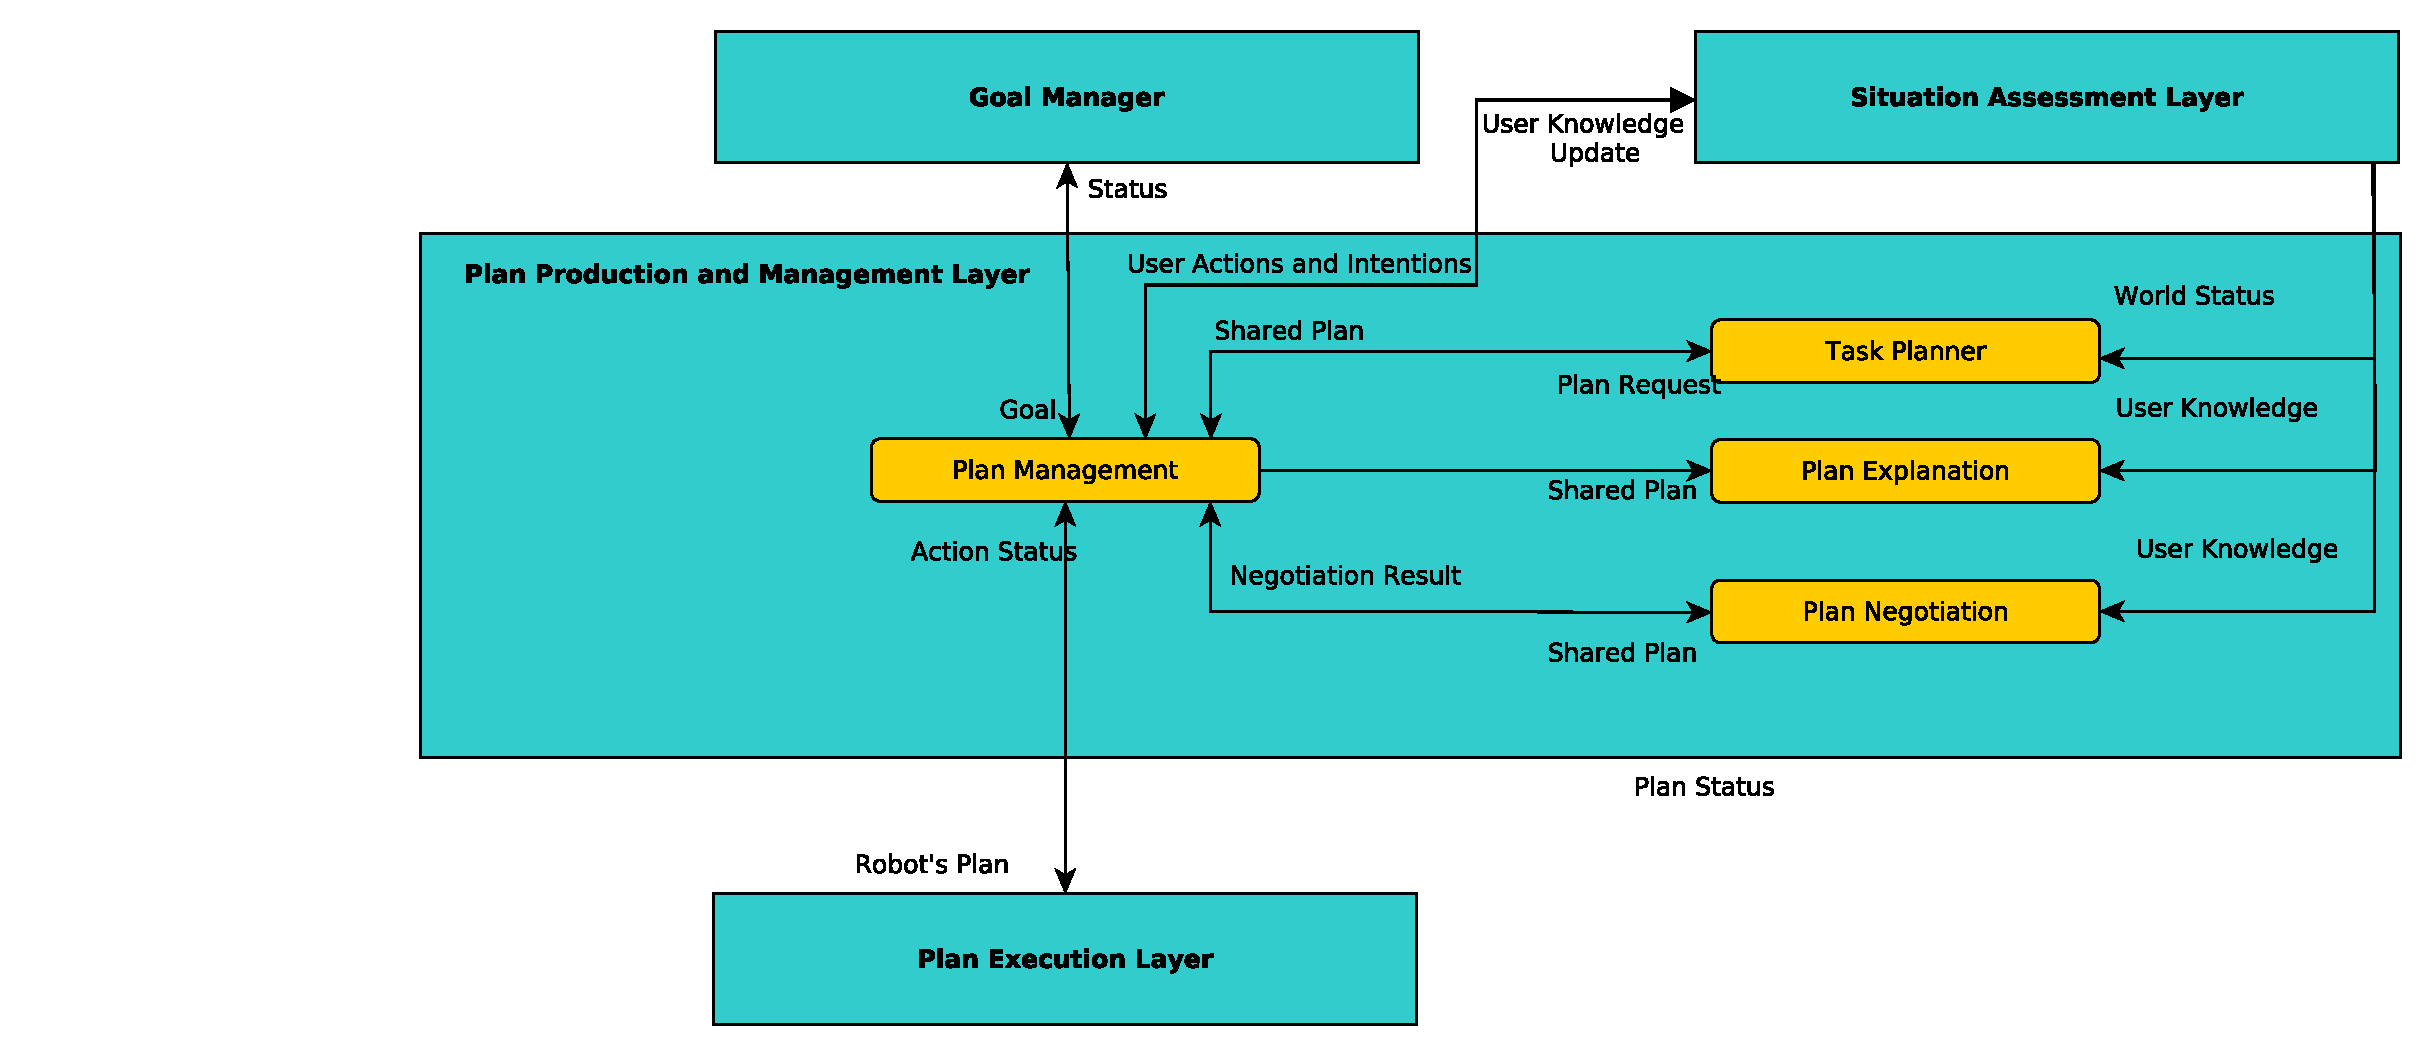
\includegraphics[clip,scale=0.6]{img/plan_management/architecture.pdf}
	\caption{The image represents the architecture of the plan management layers. Yellow rounded rectangles represent modules, while blue rectangles layers. Arrows represent message exchanged between components, with the label detailing the message. }
	\label{fig:goal_management-goal_cycle}
\end{figure}


Part of this chapter was presented in \cite{Lallement2014,milliez2016using,fioreiser2014}.

\section{Plan Management Modalities}
\label{sec-plan_management-modalities}
When acting together, agents sometimes do not have the same decision power, with one of them assuming the role of a leader. We represent this idea, in our system, by proposing three different modalities: Robot Leader, Human Leader, and Equal Partners. The robot is able to switch from one modality to another during the execution of a plan. For example, if the current modality is 'Robot Leader' and the Robot receives a command from a user, it will switch to the 'Human Leader' modality, after interrupting its current action.

\subsection{Robot Leader}
In this modality the robot, after computing the plan, will explain it, negotiate it and start executing it.
The robot will track the status of humans, informing them of which actions they should execute. This modality can be helpful when interacting with  naive users or in tasks where the robot has a better knowledge of the
domain or of the environment than the other agents.

\subsection{Human Leader}
The human can also create plans, interacting with the robot by using a
tablet application, as explained in chapter \ref{sec:situation_assessment-communication}. In this modality the robot   will simply observe the surroundings and wait for user inputs. This modality is always available and has a priority over
the other two modalities. If the robot receives a command from the
application while it is in another modality, it will abandon its current
plan, stopping its actions at a safe point, and then execute the users'
command. We feel that this interaction modality is important for two
different reasons.  First, some users will simply prefer to be in
charge of the execution process, for a matter of personal preference or because they
feel they have a deeper knowledge on how to realize the current task
than the robot. We can picture, for example, industrial or medical
scenarios, where the human is the leader and asks the robot to perform
different tasks to help him, when needed. A second use of this modality is in situations where
the robot doesn't have  a clear estimation of the users' intentions and
goals. For example, in a domestic environment, a user could decide to
order a robot to bring him a drink, a need that the robot can't always anticipate.

\subsection{Equal Partners}
In the last presented operation modality the robot will try to help
the human to complete a task. At the start of the scenario, the robot
will stand still and observe the environment. After the user takes an
action the robot will calculate a plan and try to help as it can, by
performing actions related to that task and by giving helpful information to
the user, for example to fill gaps in their knowledge. In this modality, 
the robot will not explain or negotiate the current plan.


This modality corresponds to what we feel is a very natural way of
interaction between different partners, in particular in non-critical
tasks, where defining an accurate plan between the partners is not
fundamental. 


\section{Plan Generation}
\subsection{Human-Aware Task Planner}
Hierarchical Task Network (HTN) planning is a popular approach that cuts down on the classical planning search space
by relying on a given hierarchical library of domain control knowledge. This provides an intuitive methodology for
specifying high-level instructions on how robots and agents should perform tasks, while also giving the planner enough 
flexibility to choose the lower-level steps and their ordering. In this paper we present the HATP (Hierarchical Agent-
based Task Planner) planning framework which extends the traditional HTN planning domain representation and seman-
tics by making them more suitable for roboticists, and treating agents as “first class” entities in the language. The for-
mer is achieved by allowing “social rules” to be defined which specify what behaviour is acceptable/unacceptable by
the agents/robots in the domain, and interleaving planning with geometric reasoning in order to validate online–with
respect to a detailed geometric 3D world–the human/robot actions currently being pursued by HATP.1
The planning algorithm of HATP has also been extended in various ways. First, it incorporates a simple mechanism
to take into account the (user-defined) cost of executing actions, so that instead of returning the first arbitrary solution
found, it keeps searching until an optimal (least-cost) one is found.2 Second, HATP has been extended to be more
suitable for Human-Robot Interaction (HRI); in particular, “social rules” can be included by the user to define what
the acceptable (and unacceptable) behaviours of the agents are. Two examples are: what sequences of steps should be
avoided in final solutions, and a limit on the amount of time a person should spend waiting (and doing nothing). The rules
are then used to filter out the primitive solutions found that do not meet the constraints.

%FINALE To compute collaborative plans, we use HATP \cite{lallement14} an HTN planner specifically designed for robotics.
%FINALE HATP comes along with specific features concerning plan generation, such as:
To compute collaborative plans, we use a modified HTN planner specifically designed for robotics.
It comes along with specific features concerning plan generation, such as:

\begin{itemize}
\item Agent based: it computes multi-agent plans with humans and robots acting.
\item Cost driven: the best (or a "sufficiently" good) plan is found sooner (using plan pruning).
\item Social rules: it refines the plans according to a set of rules designed to promote more socially acceptable plans  (e.g. effort balancing depending on human preferences and context, social conventions\ldots).
\end{itemize}

%The best plan is defined by its cost (the sum of every action's cost in the plan) but also by a set of social properties (e.g. how the workload is shared). To reduce the number of plans to compute, our planner is cost-driven : it throws away plans that are not promising. The plan is given in the form of the HTN tree decomposition and a set of streams, (one per agent). The decomposition tree is useful to keep the hierarchical structure. The streams represent the actions that each agent must carry out and the causal links to order them and ensure the synchronization, hence the streams are useful for the execution (e.g. to ensure turn taking). Figure \ref{fig:treePlan} depicts an extract of the tree decomposition of a solution plan (the example is described later).


Each action in the domain provides a function that estimates its cost if added to the plan. So at any time it is possible to compute the cost of the partial plan while it is being built. Furthermore the current best plan score is stored;  if at any moment the cost of the current partial plan exceeds this score, the plan is discarded and the search continues. This plan pruning helps speed up the search for the best plan. After each plan is computed a set of filtering rules are applied to sanction plans that do not exhibit certain social behaviors. Once the best plan (note that one can limit the search to a "sufficiently" good  cost level)   is retrieved, it is sent to the supervisor in the form of an HTN tree decomposition. In addition, a set of streams of actions is elaborated; each stream represents the actions an agent (human or robot) must carry out. To ensure proper action sequencing and synchronization between agents, causal links are embedded. Besides, the plan may include joint actions allocated simultaneously to two or more agents because they need tight collaboration


\subsection{Human-Aware Probabilistic Planner}

dietterich2000hierarchical
This paper presents a new approach to hierarchical reinforcement learning based on de-
composing the target Markov decision process (MDP) into a hierarchy of smaller MDPs
and decomposing the value function of the target MDP into an additive combination of the value functions of the smaller MDPs. The decomposition, known as the MAXQ decom-position, has both a procedural semantics|as a subroutine hierarchy|and a declarative
semantics|as a representation of the value function of a hierarchical policy. MAXQ uni
and extends previous work on hierarchical reinforcement learning by Singh, Kaelbling, and
Dayan and Hinton. It is based on the assumption that the programmer can identify useful
subgoals and de
programmer constrains the set of policies that need to be considered during reinforcement
learning. The MAXQ value function decomposition can represent the value function of any
policy that is consistent with the given hierarchy. The decomposition also creates oppor-
tunities to exploit state abstractions, so that individual MDPs within the hierarchy can
ignore large parts of the state space





hauskrecht1998hierarchical
We investigate the use of temporally abstract
actions, or macro-actions, in the solution of
Markov decision processes. Unlike current mod-
els that combine both primitive actions and
macro-actions and leave the state space un-
changed, we propose a hierarchical model (using
an abstract MDP) that works with macro-actions
only, and that significantly reduces the size of the
state space. This is achieved by treating macro-
actions as local policies that act in certain regions
of state space, and by restricting states in the ab-
stract MDP to those at the boundaries of regions.
The abstract MDP approximates the original and
can be solved more efficiently. We discuss sev-
eral ways in which macro-actions can be gen-
erated to ensure good solution quality. Finally,
we consider ways in which macro-actions can be
reused to solve multiple, related MDPs; and we
show that this can justify the computational over-
head of macro-action generation.


\subsection{Adapting Plan Generation to Human Knowledge}
To take knowledge into account while planning, a new social rule was needed. The aim is to select the best suited plan for the given policy. We propose two policies: favor teaching, so the human can learn from the robot, or efficiency. With the teaching policy, the planner tries to produce plans maximizing the number of human tasks where they have the opportunity to learn, while efficiency makes the planner select plans with the least amount of unknown tasks for the human in order to ensure that they can be more efficient.
%(the robot however can execute some tasks unknown to the human).
In case of a policy to favor efficiency, the rule is simply to apply a penalty every time the human has to perform an action they ignore. This penalty would be reversed for the teaching rule.

To illustrate our planner and the new social rule let us consider the toy example where a human and a robot have to cook an apple pie. A part of the solution plan is shown in Figure \ref{fig:treePlan}. In this context we can consider that the human knows how to carry out all the actions (pick, place, cut, and so on) but they may not know the exact order of steps (higher level task). If we favor teaching, the plan should contain a way to achieve the recipe with a minimal knowledge level on each task and, as much as possible, human will be in charge of those steps. On the other hand, if we favor efficiency the plan should contain the smallest amount of unknown tasks to be performed by the user.
Using this rule, the robot is able to adapt its plan generation to the knowledge of the user concerning tasks contained in the shared plan.
%, and the tasks can be carried by either of the agents. The one to be actually chosen will depend on the rest of the plan (optimality of the task allocation).
To properly compute the cost of a plan, the planner will also consider a task knowledge as upgraded once it is added to the plan. This allows the efficiency policy to prefer plans that reuse the same task many times and assign it to the same user to lower the cost, over some plans where different tasks are performed or the same task is performed by a different agent.

The planner is integrated in a dialog system that allows to negotiate plans (see below). More precisely it allows for asking about user preferences and abilities. If the user tells the system that she/he cannot perform a given task, it will not be added to the plan (invalidate the corresponding task precondition).
Concerning user preferences, the negotiation step will update a database with the preferences expressed by the user. If the user specifies that she/he (does not) want to perform certain tasks, those tasks if added to the plan, will take an important reward (resp. penalty) cost. Hence plans which contain such tasks will be considered as unwanted, however if they are the only possible solutions (because of inability and so on) they will be kept and the planner will return the one with the least number of unwanted and maximum number of wanted tasks.


\section{Plan Explanation}



% intro
%FINALE Once the robotic system has generated a collaborative plan adapted to the chosen HATP policy (about learning, abilities and preferences), the plan must be shared with the human partner.
Once the robotic system has generated a collaborative plan adapted to the chosen policies (about learning, abilities and preferences), the plan must be shared with the human partner.
Speech is a ``potent modality for the on-going maintenance of cooperative interaction'' \cite{Lallee2013}. Indeed, Tomasello even suggests that the principal function of language is to establish and negotiate cooperative plans \cite{tomasello2005}.
Considering this, we decided to use speech to present the plan to the collaborator.

\subsection{Plan Preprocessing}
The HTN tree generated represents a solution to achieve the goal. However, it may not be suitable to present or explain it like it is to the collaborator, as it may contain refinement steps that would make the explanation unclear. To adapt the plan for explanation we use two rules.
%
(1) We remove the recursive tasks. If a node $n$ of the HTN tree contains the same method (using $compare$ function) as its parent $parent(n)$, it will be replaced in the tree by its children $children(n)$. (2) We also replace nodes with a single child by their children.
\begin{enumerate}
\item $\textbf{if}$ $(compare(n, parent(n)))$ \textbf{then} $n \leftarrow children(n)$
\item $\textbf{if}$ $(children(n).size() = 1)$ \textbf{then} $n \leftarrow children(n)$
\end{enumerate}
These rules build a lighter plan tree to process.


\subsection{Plan Presentation}
%Miki: Could simplyfi in which agents are in charge of the task, removing the parhentesis.

Before executing the plan, the robot will present the goal and the proposed allocation of high-level tasks to give a global view on the plan. Standard NL generation is used as shown in Table \ref{table:pie-present}. 
To ensure the scalability of the system, when presenting the plan, the robot will verbalize only the $N$ first highest level tasks. For simplicity, we have chosen $N$=$3$ based on some runs carried out during the development process. We believe that this number would require further investigation depending on the domain or on the user and her/his confidence in the execution of the tasks. The robot will present the first steps of the plan, and then execute them. Once this execution is achieved, it will repeat the present/negotiate/execute process until the plan is completed or aborted.

% Put in a double colomn table
%\begin{tabular}{ll}
%   agents(root) $+$ have\_to $+$ root  & "We have to cook an apple pie." \\
%   introduce\_presentation & "I will tell you the steps." \\
%   agents(root.child[0]) $+$ first $+$ root.child[0] & "You will first fetch the ingredients," \\
%   then $+$ agents(root.child[1]) $+$  root.child[1] & "Then I will assemble the apple pie," \\
%   finally $+$ agents(root.child[2]) $+$  root.child[2] & "Finally you will bake the apple pie in the oven." \\


%\end{tabular}
 
 
 \begin{table}
 %\vspace{-10pt}
\centering
\scriptsize
\renewcommand{\arraystretch}{1.3}
\begin{tabular}{c|c}
   agents(root) $+$ have\_to $+$ root  & "We have to cook an apple pie." \\
   \hline
   introduce\_presentation & "I will tell you the steps." \\
   \hline
   agents(child[0]) $+$ first $+$ child[0] & "You will first fetch the ingredients," \\
   \hline
   then $+$ agents(child[1]) $+$  child[1] & "Then I will assemble the apple pie," \\
   \hline
   finally $+$ agents(child[2]) $+$  child[2] & "Finally, you will bake \\
   & the apple pie in the oven." \\
\end{tabular}
 \vspace{-4pt}
\caption{Presentation of a plan to cook an apple pie. Root is the root of the tree and child is a list with its children.}
 \vspace{-20pt}
 \label{table:pie-present}    
\end{table}
 
\section{Adaptive Plan Execution}
\label{planExecution}

\subsection{Plan Management Algorithm}
\label{sec:algo}
Once the plan has been accepted by the collaborator, the execution can start. We give the algorithm for the adaptive plan execution, and then explain it.



%    \vspace{-12pt}
% \begin{program}
% \mbox{\textbf{$execute\_tree$ algorithm:}}
% %\seq{node parent, list<node> currentNodes};
% \FOR $n:=nodes.start$ \TO $n:=nodes.end$
%      $verbalize(n)$;
%      \IF $agents(n) = {robot}$
%         \THEN \IF $children(n)$ \neq \emptyset \AND $userKn(n) = NEW$
%         \AND $teachPolicy$
%           \THEN $execute\_tree(children(n))$;
%           $userKn(n) := BEGINNER$;
%         \ELSE $execute(n)$;  \FI
        
%      \ELSIF $userKn(n) = NEW$
%        \THEN $explain(n)$;
%          \IF $children(n)$ \neq \emptyset
%            \THEN $execute\_tree(children(n))$;
%                  $userKn(n) := BEGINNER$;
%          \ELSE $monitor(n)$; \FI
         
%      \ELSIF $userKn(n) = BEGINNER$
%        \THEN \IF $proposeExplain(n)$
%            \THEN $userKn(n) = NEW$;
%            (...);\rcomment{\textit{//Same process as NEW}}
%            \ELSE $monitor(n)$; \FI
%    %          userKn(n) = INTER; \FI
             
%        \ELSIF $userKn(n) = INTERMEDIATE$ 
%        \OR $userKn(n) = EXPERT$)
%          \THEN monitor(n); \FI
%  %        \IF(userKn(n) = INTER)
%  %          userKn(n) = EXPERT; 
% %\rcomment{This text will be set flush to the right margin}
% \end{program}
%    \vspace{-5pt}



%\begin{algorithm}
\begin{algorithmic}[1]
\For{n$:=$nodes.start to n$:=$nodes.end}
	\If{$agents$(n) = \{robot\}}\label{alg:onlyRobotStart}
    	\If{$children(n) \neq \emptyset$ $\wedge$ $user\_kn(n)$ = NEW\par
        \hskip\algorithmicindent $\wedge$ $teachPolicy$}
        	\State $execute\_tree(children(n))$
            \State $user\_kn(n) :=$ BEGINNER
        \Else
         	\State $execute(n)$
        \EndIf\label{alg:onlyRobotEnd}
    \ElsIf{$user\_kn(n)$ = NEW}\label{alg:newStart}
     	\State $explain(n)$
        \If{$children(n)$ $\neq \emptyset$}
          	\State $execute\_tree(children(n))$
            \State $user\_kn(n)$ $:=$ BEGINNER
        \Else
         	\State $monitor(n)$
        \EndIf\label{alg:newEnd}
    \ElsIf{$user\_kn(n)$ = BEGINNER}\label{alg:beginnerStart}
      	\If{$propose\_explain(n)$}
          	\State $user\_kn(n)$ $:=$ NEW
            \State $(\dots)$ \Comment{Same process as NEW}
        \Else
          	\State $monitor(n)$
        \EndIf\label{alg:beginnerEnd}
    \ElsIf{$user\_kn(n)$ = INTERMEDIATE\par
    \hskip\algorithmicindent $\vee$ $user\_kn(n)$ = EXPERT}\label{alg:interStart}
      	\State $monitor(n)$
    \EndIf\label{alg:interEnd}
\EndFor
\end{algorithmic}
%\caption{$execute\_tree(n)$}

%\end{algorithm}



\begin{itemize}
\item \textit{$execute\_tree(n)$} is the main function to manage the execution. This is called after the negotiation process. It has \textit{$nodes$}, a list of nodes initially filled with the root's children, as an argument.
\item \textit{$teachPolicy$} is a boolean to define if we are in teaching or efficient mode.
\item \textit{$agents(n)$} returns the agents involved in the node \textit{n}.
\item \textit{$verbalize(n)$} will verbalize the current task, using the node context to present it (e.g. using sequential relations such as first, then or finally according to the node position in the list).
\item \textit{$user\_kn(n)$} returns the knowledge level of the user concerning the task \textit{n}.
\item \textit{$propose\_explain(n)$} will lead the robot to propose an explanation for the current task. If the user accepts the explanation it will return true, and otherwise false.
\item \textit{$explain(n)$} launches a procedure to explain the current task to the user. This procedure could be implemented as a script to launch a video, an explanation speech or even to ask an expert to explain the task.
\item \textit{$monitor(n)$} sends a request to the supervision system to monitor proper execution of the current node. If the request returns a success, the function will upgrade the user's knowledge and \textit{$execute\_tree$} function will continue. In case of failure, the function will downgrade the user's knowledge, exit the \textit{$execute\_tree$} function, and return a failure that will result in a replan request to the supervisor and a new execution if a plan is found.
\item \textit{$execute(n)$} works in a similar way to the monitor but sends a request to execute the node by the robot.
\end{itemize}
 
\subsection{Explanation of the plan management algorithm}
During the execution, we use the HTN processed tree to execute the plan, give explanation about tasks and monitor them according to the knowledge values in the user model.
We use a depth first plan exploration process to proceed with the execution as it gives context to the task to perform.
When reaching a node, several situations may occur.
% Monitor function is responsible for: knowledge update(success = upgrade, fail = downgrade) and replan in case of failure. 

\subsubsection{Only the robot is involved (lines ~\ref{alg:onlyRobotStart}-~\ref{alg:onlyRobotEnd})} if the robot is the only agent in charge of the current node, if the collaborator has a knowledge level equal to \textit{NEW} for the current task and the chosen policy for the interaction is teaching, the robot will execute the subtasks in ``demonstration mode'', meaning that it will verbalize each child task before performing it. Once it's done, the robot updates the human's knowledge on the current node to \textit{BEGINNER}. The same process will be applied to the children, so the robot will verbalize each (and only) task that needs to be learned by the collaborator.
If the robot is in charge, but the human collaborator already has knowledge on the task, or the current policy is efficiency, the robot will verbalize only the high-level task it performs.

Then, if the human is involved in the current node, the robot's behavior will depend on the human's knowledge level for the task, as it may have to explain it.
The explanation could be done in several ways: showing a video, asking an expert to explain the task or simply verbally guiding the user, step by step. We will provide details about verbally guiding the user since it is the one actually involving the robot. 

% if new
\subsubsection{The collaborator is \textit{NEW} (lines~\ref{alg:newStart}-~\ref{alg:newEnd})} if the human has a level NEW for the current task, we explain it.
When verbally guiding the user, if the current node has only one child node, we  go deeper in the tree and apply again the corresponding behavior according to the knowledge level. If the current node is actually an operator (a leaf), the supervisor waits for the user to perform the current action. In case of success, the knowledge level for the task is upgraded to \textit{BEGINNER} (in the above algorithm this is done in the \textit{monitor} process).

% if beginner
\subsubsection{The collaborator is \textit{BEGINNER} (lines ~\ref{alg:beginnerStart}-~\ref{alg:beginnerEnd})} if the human has a level \textit{BEGINNER} for the current task, we ask if he needs explanation. If so, we downgrade his knowledge level to NEW, on the current task, and apply the same process as the previous level. If the user refuses explanations, we simply monitor the execution of the current node. In case of success, the knowledge level for the current task is upgraded to \textit{INTERMEDIATE}. This knowledge level will also be used as default. This way, when we don't know the knowledge level of an agent concerning a task, we just ask him if he needs an explanation and adapt the behavior accordingly.

% if intermediate
\subsubsection{The collaborator is \textit{INTERMEDIATE} (lines~\ref{alg:interStart}-~\ref{alg:interEnd})} if the human has a level \textit{INTERMEDIATE} for the current task, we verbalize it without proposing explanations, since he has already  succeeded with the plan at least once without help. Also, we do not go deeper in the tree and directly monitor the current task. If the user  fails, we downgrade his knowledge to \textit{BEGINNER}, otherwise we upgrade it to \textit{EXPERT}.

% if expert
\subsubsection{The collaborator is \textit{EXPERT} (lines~\ref{alg:interStart}-~\ref{alg:interEnd})} in case of \textit{EXPERT} knowledge level on the current task, we  proceed as for the previous knowledge level, downgrading to \textit{INTERMEDIATE} if the user makes a mistake and keeping the \textit{EXPERT} level if he performs the task as expected.

\subsection{Failure and Replanning}
The goal of monitoring human actions is to be able to recover from unexpected behaviors of the human. When this happens, the robot needs to inform the human of his potentially wrong behavior and downgrade his knowledge level. Consequently, the next time the human will perform this task the robot will guide and monitor his execution at a more refined level (the children tasks).
%maybe also the dad function to unknown to regive the context?
The task planner is requested to compute a new plan to achieve the goal with the updated world state.
One of the benefits of the dynamical update of human knowledge is that this new plan may have tasks that the robot has already explained or that the human has performed before the failure occurred. In this case, guiding the human through the new plan execution will be faster as the robot will not have to reexplain these tasks. 
This replanning behavior gives robustness to the robotic system and allows a socially acceptable recovery procedure where we inform the human with the error and reexplain the plan only at the needed level of detail.

\section{Plan Negotiation}
Once the robot has presented the main tasks and repartition, it has to ensure that the human agrees with this shared plan. The robot will simply ask the human for approval and inquire what is wrong in case of disagreement.
In the current version of our system, two kinds of human requests are handled. First the user can express her/his preferences, either the will to perform a task previously assigned to the robot or the denial to perform a task assigned to her/him. The other possibility is to inform the robot that the user cannot perform an action. This will be added to the user's model and stored in the database. The robot will then try to find a new plan that prevents the human from performing a task the user is not willing or able to perform. This plan will then be presented and the robot will ask again for the user's approval. In our system, the user's preferences have a higher cost than the teaching policy as we consider that the user should have the final decision.



\section{Plan Monitoring}
During the execution of a plan, the robot will monitor other agents. In general, having a shared plan, the robot knows what is the user next expected action, and can monitor if it's accomplished. In general plan monitoring poses a number of different issues:
\begin{itemize}
\item Understanding when the next expected action has been performed. In some situations the robot will monitor the execution of a specific action. In this event, it needs to understand when the action has been performed.
\item Understanding when the next expected task has been performed. In some situations, the robot wants to give a human cooperator the freedom to perform a subtask has it sees fit. This is a more complext problem than monitoring a specific action, since the robot needs to reason on the results of a sequence of actions.
\item Evaluating the human engagement in the current task. The robot needs to understand if the human is trying to accomplish its current task, if he momentarily interrupted it, or if he abandoned it.
\end{itemize}

\subsection{Monitoring at Action Level}
The robot can be updated at each time on what actions have been performed, using the mechanisms described in the Situation Assessment chapter. This way, the robot can compare the actions performed by humans, with those that should be performed following the shared plan.

\subsection{Monitoring at Task Level}
Monitoring an expected task is a more complex issue, as humans have several way to complete it. We can deal with this issue by using the ideas presented in the Intention Recognition paper with the hierarchical MDP models presented here. In general, the Intention Recognition model will be inferring human intentions from a known list of possible intentions, which should include the possible goals in the system, and so the shared goal that is been performed with the robot. We add a new intention to monitor, assigned to the HMDP related to the subtask assigned to the user, with the same contexts as the high-level intention, and monitor his engagement level.

 If the Intention Recognition module detects that the human's intention correspond to the current task, than the robot will consider that the human is proceeding with his part of the plan. When this intention will be achieved, the robot will start to monitor the next task assigned to the human.

\subsection{Evaluating Human Engagement}
Human Engagement in a task can be evaluated using the Intention Recognition framework. %%Add the previous part

\subsection{Adapting Monitoring to Human Knowledge}
Once the current task to perform has been explained, the robot performs it if it is allocated to it, or it  monitors its human partner's task performance. Consequently, the monitoring may be done at high-level tasks if the human has enough knowledge of it.
We have chosen this adaptive way of monitoring since we believe the robot would be more efficient, sparing its resources, by focusing its attention more often on parts of the plan that have never been performed by the human partner, and less when he has some form of expertise, leaving more freedom to the human on the way to execute tasks he knows.

Monitoring human actions is complex, particularly with high-level tasks, where we are not monitoring a set of atomic actions. The system should have reasoning models for the robot to understand if the state of the world is coherent with the action that the human needs to perform. It should also be able to measure the level of engagement of the human to the task, in order to better assess if the human is executing or not his part of the shared plan, and to react accordingly.

\subsection{Monitoring and Unseen Actions}
Often, in cooperative tasks, the agents will operate in different locations, and so their actions won't be observable at all time. Perhaps one of the agents is preparing a cake in the kitchen,  while the robot is preparing the table. While we don't deal, in this work, with these issues, there are studies on plan recognition in partially observable environments. %CITA


\subsection{Failed Monitoring and Replanning}
What happens when a human is not engaged in the current task? There are three possibilities:
\begin{itemize}
\item The human is momentarily doing another task: in this case, the robot will simply wait, without considering the human's assigned task as failed.
\item The human is engaged in a different long-term task, related to the current scenario: in this case, the robot will act differently depending on the 
current modality. In the 'robot leader' mode, the robot will issue a warning to the human. In the 'Equal Partners' or 'Human Leader' modalities, the robot will create a new plan, and try to adapt to the human.  %%What should the robot actually do?
\item The human is engaged in a different long-term task, not related to the current scenario. In this case, the robot will create a new plan, not considering the human as a partner.
\end{itemize}

To understand if a task is 'short term' or 'long term' we can hand-code these information, linking it to the intentions. We infer that a human is engaged in a different task, but still related to the same scenario, if the likelihood that the human intention is its assigned task is low, but the likelihood that the human intention is the shared goal is still high. 



